\documentclass[12pt]{article}
\usepackage{amsmath}
\usepackage{amssymb}
\usepackage{tikz}
\usetikzlibrary{matrix, positioning}

\begin{document}

\begin{figure}[h]
    \centering
    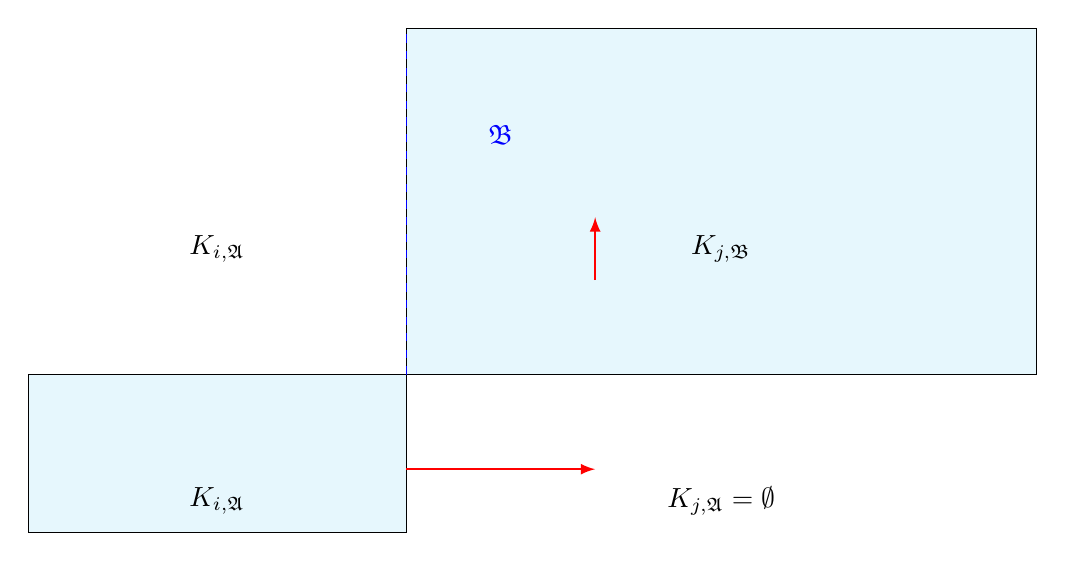
\begin{tikzpicture}[scale=0.8]
        % Cells
        \draw[fill=cyan!10] (-3,-1.5) rectangle (7,4);
        \draw[fill=white] (-3,-4) rectangle (-9,-1.5);
        \draw[fill=cyan!10] (-9,-1.5) rectangle (-3,-4);

        % Species labels
        \node at (-6, 0.5) {$K_{i,\mathfrak{A}}$};
        \node at (2, 0.5) {$K_{j,\mathfrak{B}}$};
        \node at (2, -3.5) {$K_{j,\mathfrak{A}} = \emptyset$};
        \node at (-6, -3.5) {$K_{i,\mathfrak{A}}$};

        % Interface
        \draw[dashed, blue] (-3, -1.5) -- (-3, 4);
        \draw[red, thick, -latex] (-3, -3) -- (0, -3);
        \draw[red, thick, -latex] (0, 0) -- (0, 1);

        % Species label above the interface
        \node[above, blue] at (-1.5, 2) {$\mathfrak{B}$};
    \end{tikzpicture}
    \caption{Illustration of the species coupling in case of a coinciding interface. In the figure, the dashed interface lies on top of the edge between two cells. It is assumed that $K_j$ in Equation~\ref{eq:coinFrac} is the cell with the lower index and owns the coinciding interface. The affected edge $\partial K_i \cap \partial K_j$ belongs to the species $\mathfrak{A}$ and takes care of the coupling between cells $K_{i,\mathfrak{A}}$ and $K_{j,\mathfrak{A}}$. The species are then coupled inside $K_j$ via the interface, from the empty cell $K_{j,\mathfrak{A}} = \emptyset$ to the full cell $K_{j,\mathfrak{B}} = K_j$. Finally, by performing the agglomeration, the discrete system is algebraically modified. This modification eliminates the (edge) contributions on $\partial K_{j,\mathfrak{A}}$ of the empty cell and combines the cell and species coupling, establishing the connection between $K_{i,\mathfrak{A}}$ and $K_{j,\mathfrak{B}}$. The lower part of the figure shows an exploded view of the situation to clarify the connectivity.}
    \label{fig:coupling}
\end{figure}

\end{document}